% Compile with XeLaTeX because the report contains Persian examples.
\documentclass[12pt,a4paper]{article}

\usepackage[margin=1in]{geometry}
\usepackage{fontspec}
\usepackage{hyperref}
\usepackage{xcolor}
\usepackage{longtable}
\usepackage{array}
\usepackage{enumitem}
\usepackage{listings}
\usepackage{caption}
\usepackage{float}
\usepackage{tikz}
\usetikzlibrary{arrows.meta,positioning,shapes.geometric}

\setmainfont{Times New Roman}
\setmonofont{Consolas}

\definecolor{codebg}{RGB}{248,248,248}
\definecolor{codeframe}{RGB}{210,210,210}
\definecolor{linkblue}{RGB}{20,80,160}

\hypersetup{
  colorlinks=true,
  linkcolor=linkblue,
  urlcolor=linkblue,
  citecolor=linkblue
}

\lstdefinestyle{projectcode}{
  backgroundcolor=\color{codebg},
  frame=single,
  rulecolor=\color{codeframe},
  basicstyle=\ttfamily\small,
  breaklines=true,
  columns=fullflexible,
  keepspaces=true,
  showstringspaces=false
}

\lstdefinelanguage{json}{
  basicstyle=\ttfamily\small,
  showstringspaces=false,
  breaklines=true,
  morestring=[b]",
  morecomment=[l]{//},
  literate=
   *{0}{{{\color{blue}0}}}{1}
    {1}{{{\color{blue}1}}}{1}
    {2}{{{\color{blue}2}}}{1}
    {3}{{{\color{blue}3}}}{1}
    {4}{{{\color{blue}4}}}{1}
    {5}{{{\color{blue}5}}}{1}
    {6}{{{\color{blue}6}}}{1}
    {7}{{{\color{blue}7}}}{1}
    {8}{{{\color{blue}8}}}{1}
    {9}{{{\color{blue}9}}}{1}
}

\lstset{style=projectcode}

\title{MLOps Phase 2 Documentation\\Agentic AI on Phase 1 RAG}
\author{Torob Product Retrieval Project}
\date{\today}

\begin{document}
\maketitle

\begin{abstract}
This document explains the Phase 2 implementation of the MLOps project. The goal of Phase 2 is to build an Agentic AI layer on top of the Phase 1 RAG system. The agent exposes a judge-compatible \texttt{/chat} API, uses the Phase 1 product artifacts as a retrieval tool, keeps short-term conversation memory by \texttt{chat\_id}, and returns product-level and seller-level random keys in the required JSON format.
\end{abstract}

\tableofcontents
\newpage

\section{Project Location}

The Phase 2 implementation is placed in a fully separated folder:

\begin{lstlisting}
<PROJECT_ROOT>\phase2
\end{lstlisting}

The Phase 1 source and artifacts are kept in the separated \texttt{phase1} folder. Phase 2 reads the existing Phase 1 outputs from:

\begin{lstlisting}
<PROJECT_ROOT>\phase1\torob_rag\artifacts
\end{lstlisting}

\section{Requirement-by-Requirement Implementation}

\begin{longtable}{|p{0.27\textwidth}|p{0.36\textwidth}|p{0.27\textwidth}|}
\hline
\textbf{Documentation Requirement} & \textbf{Implemented Solution} & \textbf{Main Files} \\
\hline
Agent with tool use & The agent detects the user intent and calls the RAG tool when product data is required. & \texttt{agent.py}, \texttt{rag.py} \\
\hline
RAG from Phase 1 as a tool & The Phase 1 cleaned product and member artifacts are loaded and queried by a dedicated tool class. & \texttt{rag.py} \\
\hline
Short-term memory & The service stores recent messages and extracted slots by \texttt{chat\_id}. & \texttt{memory.py} \\
\hline
API endpoint for judge & The project exposes \texttt{POST /chat} with the required JSON contract. & \texttt{server.py} \\
\hline
CLI or UI & A CLI is provided, and \texttt{GET /} serves a small browser test page. & \texttt{cli.py}, \texttt{server.py} \\
\hline
Monitoring & Events and metrics are written to local runtime files. & \texttt{monitoring.py} \\
\hline
Guardrails & Prompt-injection style requests are refused, and unknown requests are answered with uncertainty. & \texttt{agent.py} \\
\hline
Test scenarios & Smoke tests and example scenarios are provided. & \texttt{tests/}, \texttt{docs/test\_scenarios.md} \\
\hline
\end{longtable}

\section{High-Level Architecture}

\begin{figure}[H]
\centering
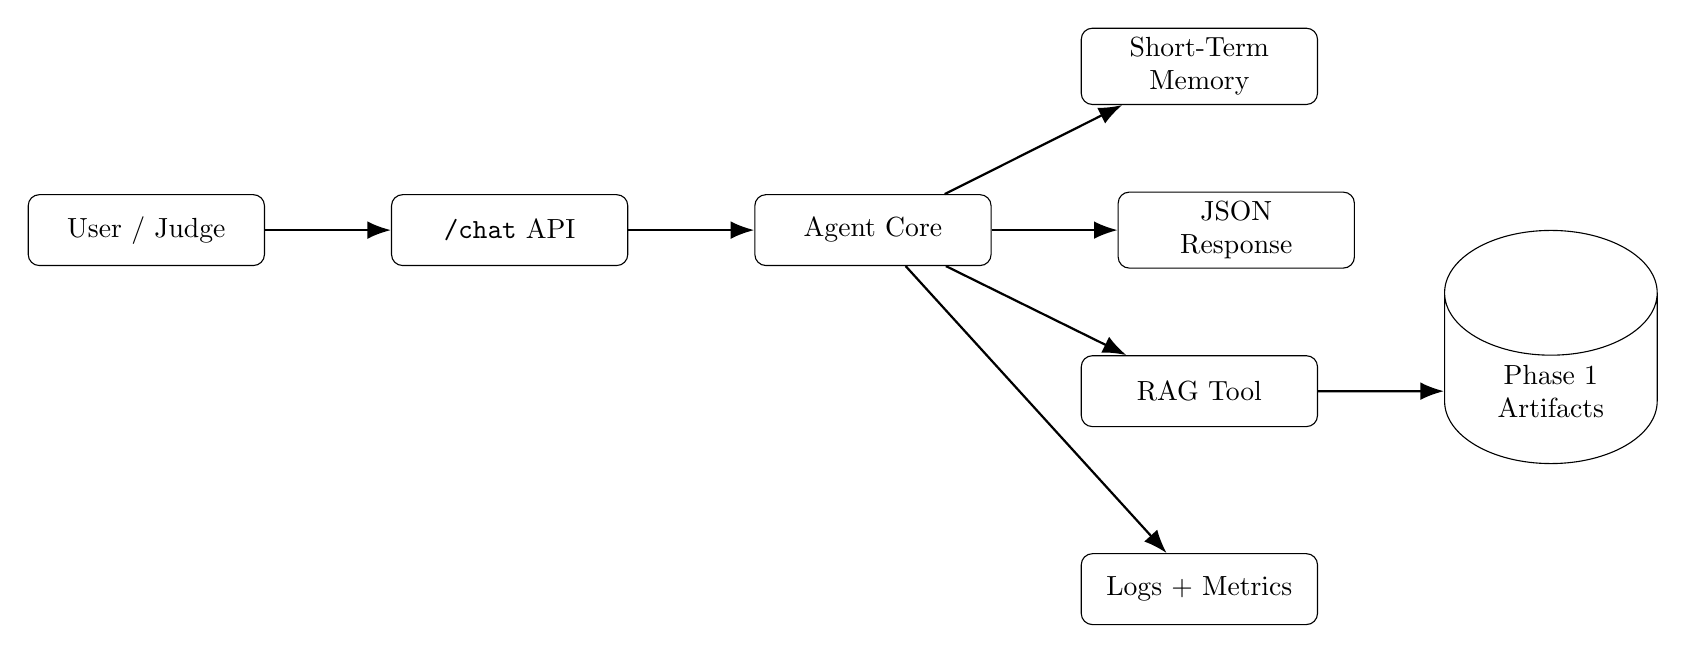
\begin{tikzpicture}[
  node distance=1.6cm,
  box/.style={rectangle, draw, rounded corners, align=center, minimum width=3.0cm, minimum height=0.9cm},
  db/.style={cylinder, draw, shape border rotate=90, align=center, minimum width=2.7cm, minimum height=1.1cm},
  arrow/.style={-{Latex[length=3mm]}, thick}
]
\node[box] (user) {User / Judge};
\node[box, right=of user] (api) {\texttt{/chat} API};
\node[box, right=of api] (agent) {Agent Core};
\node[box, above right=of agent] (memory) {Short-Term\\Memory};
\node[box, below right=of agent] (rag) {RAG Tool};
\node[db, right=of rag] (artifacts) {Phase 1\\Artifacts};
\node[box, right=of agent] (response) {JSON\\Response};
\node[box, below=of rag] (monitor) {Logs + Metrics};

\draw[arrow] (user) -- (api);
\draw[arrow] (api) -- (agent);
\draw[arrow] (agent) -- (memory);
\draw[arrow] (agent) -- (rag);
\draw[arrow] (rag) -- (artifacts);
\draw[arrow] (agent) -- (response);
\draw[arrow] (agent) -- (monitor);
\end{tikzpicture}
\caption{Phase 2 Agentic RAG architecture.}
\end{figure}

\section{Main Components}

\subsection{HTTP Server}

The HTTP server is implemented with Python's standard \texttt{http.server}. It provides four routes:

\begin{itemize}[noitemsep]
  \item \texttt{GET /}: browser-based manual test page.
  \item \texttt{GET /health}: health check endpoint.
  \item \texttt{GET /metrics}: runtime metrics endpoint.
  \item \texttt{POST /chat}: required judge endpoint.
\end{itemize}

Main file:

\begin{lstlisting}
phase2/src/agentic_rag/server.py
\end{lstlisting}

\subsection{Agent Core}

The agent receives a parsed chat request and decides which behavior is needed. The implemented intent categories are:

\begin{itemize}[noitemsep]
  \item product search,
  \item product feature question,
  \item seller or price question,
  \item multi-turn seller hunt,
  \item product comparison,
  \item image-to-base request,
  \item guardrail or out-of-scope response.
\end{itemize}

Main file:

\begin{lstlisting}
phase2/src/agentic_rag/agent.py
\end{lstlisting}

\subsection{Phase 1 RAG Tool}

The RAG tool loads real Phase 1 artifacts:

\begin{lstlisting}
phase1/torob_rag/artifacts/clean/unified_base_products.parquet
phase1/torob_rag/artifacts/clean/members_clean.parquet
phase1/torob_rag/artifacts/embeddings/clip_v1/image/image_index.parquet
\end{lstlisting}

It provides three main operations:

\begin{itemize}[noitemsep]
  \item \texttt{search\_products(query, top\_k)}: returns base products.
  \item \texttt{get\_members(base\_random\_key, intent)}: returns seller-level member products.
  \item \texttt{image\_to\_base(image\_base64)}: returns one base product key from the Phase 1 image index.
\end{itemize}

Main file:

\begin{lstlisting}
phase2/src/agentic_rag/rag.py
\end{lstlisting}

\subsection{Memory}

The short-term memory is keyed by \texttt{chat\_id}. This is important because the judge may send several consecutive requests with the same conversation id.

The memory stores:

\begin{itemize}[noitemsep]
  \item recent dialogue messages,
  \item extracted city,
  \item extracted budget,
  \item extracted style or material,
  \item extracted product intent.
\end{itemize}

Runtime memory is saved in:

\begin{lstlisting}
phase2/runtime/memory.json
\end{lstlisting}

Main file:

\begin{lstlisting}
phase2/src/agentic_rag/memory.py
\end{lstlisting}

\subsection{Monitoring}

The implementation includes lightweight local monitoring. It records:

\begin{itemize}[noitemsep]
  \item short-term and semantic memory writes,
  \item memory reads,
  \item RAG tool calls,
  \item agent responses,
  \item HTTP requests,
  \item errors.
\end{itemize}

Generated files:

\begin{lstlisting}
phase2/logs/events.jsonl
phase2/logs/metrics.json
\end{lstlisting}

Metrics include:

\begin{itemize}[noitemsep]
  \item Mean Time To Answer,
  \item Tokens Per Message,
  \item Memory Hit Rate.
\end{itemize}

\section{API Contract}

\subsection{Endpoint}

\begin{lstlisting}
POST /chat
Content-Type: application/json
\end{lstlisting}

\subsection{Request Format}

\begin{lstlisting}[language=json]
{
  "chat_id": "test-1",
  "messages": [
    {
      "type": "text",
      "content": "کمترین قیمت برای ماگ هندوانه فانتزی و کارتونی کد 1375 چقدر است؟"
    }
  ]
}
\end{lstlisting}

\subsection{Response Format}

\begin{lstlisting}[language=json]
{
  "message": "بر اساس نتایج بازیابی‌شده، کمترین قیمت ... برابر 209000 است.",
  "base_random_keys": ["hhtgaa"],
  "member_random_keys": ["pjwyvz"]
}
\end{lstlisting}

\section{How Each Required Scenario Is Handled}

\subsection{Scenario 1: Question About a Product Feature}

If the user asks about a feature such as material, capacity, width, color, or dimensions, the agent:

\begin{enumerate}[noitemsep]
  \item searches for the product in Phase 1 data,
  \item reads the \texttt{extra\_features} field,
  \item extracts the requested attribute if available,
  \item returns the answer and the related \texttt{base\_random\_key}.
\end{enumerate}

Relevant code:

\begin{lstlisting}
Agent._feature_question()
Phase1RAGTool.answer_feature()
\end{lstlisting}

\subsection{Scenario 2: Question About Sellers or Prices}

If the user asks for the cheapest seller or a seller recommendation, the agent:

\begin{enumerate}[noitemsep]
  \item maps the query to one base product,
  \item fetches member products with the same \texttt{base\_random\_key},
  \item sorts by price for cheapest queries,
  \item returns one or more \texttt{member\_random\_keys}.
\end{enumerate}

Relevant code:

\begin{lstlisting}
Agent._seller_question()
Phase1RAGTool.get_members()
\end{lstlisting}

\subsection{Scenario 3: Multi-Turn Seller Hunt}

For ambiguous seller-hunt requests, the agent first asks for more details. In later requests with the same \texttt{chat\_id}, it uses memory slots such as budget, city, and style.

Relevant code:

\begin{lstlisting}
Agent._seller_hunt()
MemoryStore.update_slots()
\end{lstlisting}

\subsection{Scenario 4: Comparing Products}

For comparison questions, the agent searches each mentioned product and selects the product that best matches the stated use case.

Relevant code:

\begin{lstlisting}
Agent._compare()
Agent._choose_product()
\end{lstlisting}

\subsection{Scenario 5: Image to Base}

For image requests, the system accepts a Base64 image message and returns one base product key from the Phase 1 image index. This keeps the required API behavior available without adding a heavy VLM dependency.

Relevant code:

\begin{lstlisting}
Agent._image_response()
Phase1RAGTool.image_to_base()
\end{lstlisting}

\section{Guardrails}

The agent refuses requests that try to reveal system prompts or hidden context. If the question is outside the product retrieval domain, the response says that the system is not confident because the question is outside the Phase 1 product data.

Relevant code:

\begin{lstlisting}
Agent._is_injection()
Agent.chat()
\end{lstlisting}

\section{How to Run}

\subsection{Install Requirements}

From the project root:

\begin{lstlisting}
cd "<PROJECT_ROOT>\phase2"
pip install -r .\requirements.txt
\end{lstlisting}

\subsection{Start the Server}

\begin{lstlisting}
$env:PHASE1_ARTIFACTS_DIR = "..\phase1\torob_rag\artifacts"
python .\run_server.py --host 127.0.0.1 --port 8000
\end{lstlisting}

Expected output:

\begin{lstlisting}
Phase 2 Agentic RAG is running at http://127.0.0.1:8000
Use POST /chat. Press Ctrl+C to stop.
\end{lstlisting}

\subsection{Browser Test Page}

Open:

\begin{lstlisting}
http://127.0.0.1:8000/
\end{lstlisting}

The page provides a small form that sends the message to \texttt{/chat}.

\subsection{Health Check}

\begin{lstlisting}
http://127.0.0.1:8000/health
\end{lstlisting}

Expected result:

\begin{lstlisting}[language=json]
{"status": "ok"}
\end{lstlisting}

\section{How to Test}

\subsection{Built-in Tests}

\begin{lstlisting}
$env:PHASE1_ARTIFACTS_DIR = "..\phase1\torob_rag\artifacts"
python .\tests\smoke_test.py
python .\tests\http_smoke_test.py
\end{lstlisting}

\subsection{Presentation Demo}

The presentation demo starts a temporary \texttt{/chat} server, sends the main evaluation scenarios as real HTTP requests, validates the expected response fields, prints each request/response pair, and stops the server automatically.

\begin{lstlisting}
python .\tests\presentation_demo.py
\end{lstlisting}

\subsection{Manual PowerShell Test}

\begin{lstlisting}
$body = @{
  chat_id = "test-1"
  messages = @(
    @{
      type = "text"
      content = "کمترین قیمت برای ماگ هندوانه فانتزی و کارتونی کد 1375 چقدر است؟"
    }
  )
} | ConvertTo-Json -Depth 5

Invoke-RestMethod `
  -Method Post `
  -Uri "http://127.0.0.1:8000/chat" `
  -ContentType "application/json; charset=utf-8" `
  -Body ([System.Text.Encoding]::UTF8.GetBytes($body))
\end{lstlisting}

\section{Example Outputs}

\subsection{Seller Price Example}

Input:

\begin{lstlisting}
کمترین قیمت برای ماگ هندوانه فانتزی و کارتونی کد 1375 چقدر است؟
\end{lstlisting}

Output:

\begin{lstlisting}[language=json]
{
  "message": "بر اساس نتایج بازیابی‌شده، کمترین قیمت برای «خرید ماگ-لیوان هندوانه فانتزی و کارتونی کد 1375» برابر 209000 است.",
  "base_random_keys": ["hhtgaa"],
  "member_random_keys": ["pjwyvz"]
}
\end{lstlisting}

\section{Limitations}

\begin{itemize}
  \item The text retrieval is a simple lexical search over the Phase 1 cleaned product table. This keeps the service easy to run on the current machine.
  \item The image scenario returns a base key from the existing Phase 1 image index but does not run a heavy CLIP/VLM model at request time.
  \item No external LLM API key is required. The response generation is deterministic and based on retrieved evidence.
  \item The first startup may take some time because the real Phase 1 parquet files are loaded.
\end{itemize}

\section{Conclusion}

The Phase 2 implementation satisfies the core project goals with a simple and runnable design. It wraps the Phase 1 RAG artifacts as a tool, provides the required \texttt{/chat} endpoint, maintains short-term memory by \texttt{chat\_id}, returns base and member random keys in the required format, and includes lightweight monitoring and tests.

\end{document}
